    % This file is part of nrf_seminar.

    % nrf_seminar is free software: you can redistribute it and/or modify
    % it under the terms of the GNU General Public License as published by
    % the Free Software Foundation, either version 3 of the License, or
    % (at your option) any later version.

    % nrf_seminar is distributed in the hope that it will be useful,
    % but WITHOUT ANY WARRANTY; without even the implied warranty of
    % MERCHANTABILITY or FITNESS FOR A PARTICULAR PURPOSE.  See the
    % GNU General Public License for more details.

    % You should have received a copy of the GNU General Public License
    % along with nrf_seminar.  If not, see <https://www.gnu.org/licenses/>.

\begin{textblock}{7.}(0., -4.)
    \begin{itemize}
        \item Synthesis of heavy elements in the universe
        \item Competition between photoabsorption (photodisintegration) and neutron capture
    \end{itemize}
\end{textblock}

\begin{textblock}{9.}(0., 3.)
    \textit{Schematic figure that shows the competition between neutron capture and photodisintegration in the r-process.
    I chose a figure from a textbook by C. Iliadis.}
    %\includegraphics[width=\textwidth]{figures/r_process_schematic.pdf}
\end{textblock}

\begin{textblock}{7.}(8., -4.)
    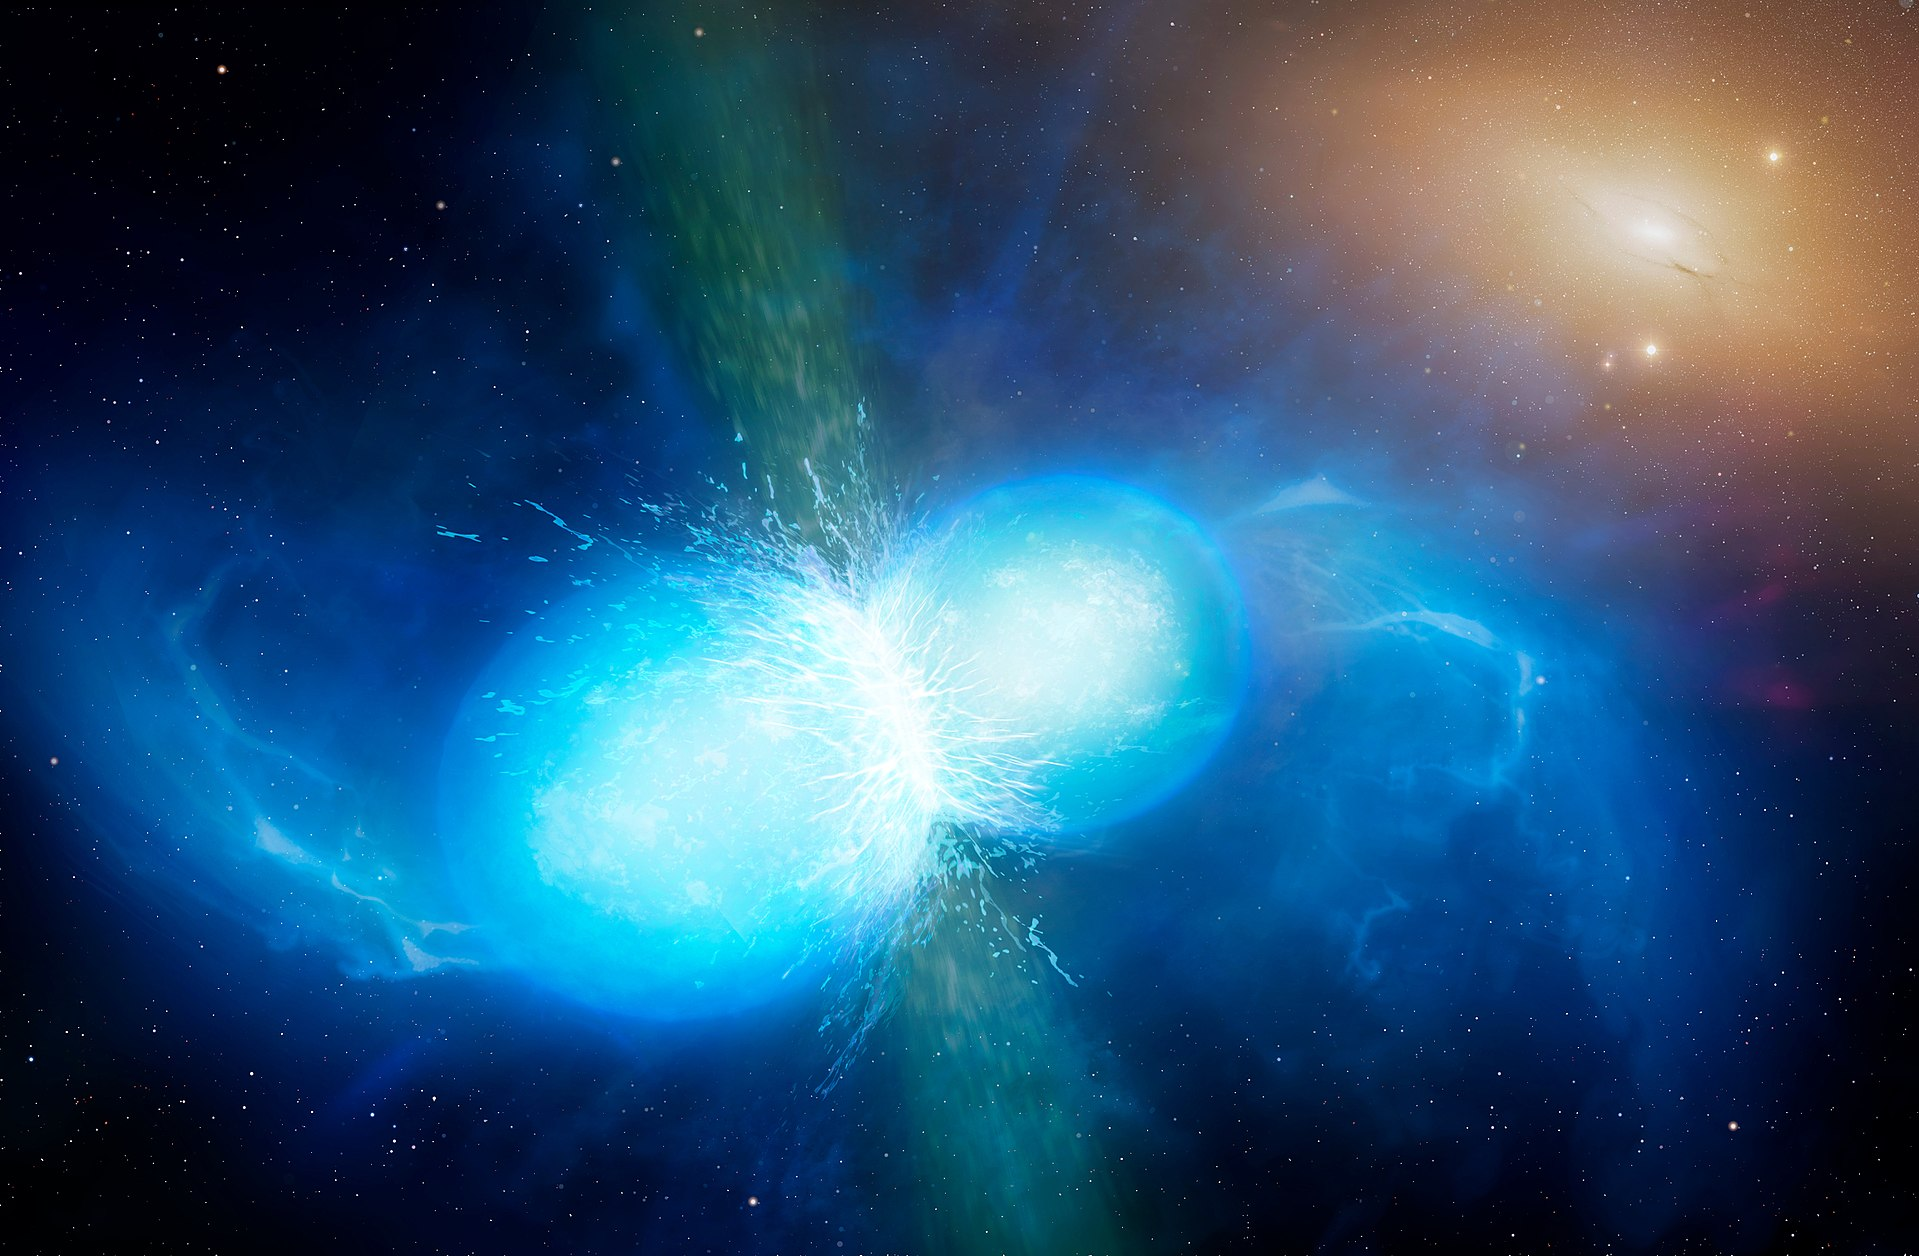
\includegraphics[width=\textwidth]{figures/neutron_star_merger.jpg}
\end{textblock}